\chapter{Replication}
In this section, we will analyze the \textbf{replication of data}, considered also as the \textit{management of a set of data} copies among multiple computers.

The motivations that lead us to discuss about this specific topics are the following:
\begin{itemize}
    \item \textbf{Availability:} users require services to be highly available. The factors that are relevant to high availability are:
    \begin{itemize}
        \item \textit{Server failures:} in this case replication is a technique for automatically maintaining the availability of data despite server failures.
        \item \textit{Network partitions and disconnected operation:} mobile users may deliberately disconnect their computers or become unintentionally disconnected from a wireless network as they move around.
    \end{itemize}
    \item \textbf{Fault tolerance:} a fault-tolerant service always guarantees \textit{strictly correct behavior} or data despite a certain number and type of \textbf{faults}.
    \item \textbf{Performance:} the caching of data at clients and servers is by now familiar as a means of performance enhancement.
\end{itemize}

Traditionally, in a distributed system, data are shared among several machines, for this reason, processes can work on different copies distributed in a \textbf{data store}. \textbf{Consistency models} can be considered as special agreements between processes and data store.

\section{Consistency models}
\textbf{Consistency models} specifies a \textbf{contract} between \textit{programmer} and \textit{system}, wherein the system guarantees that if the programmer follows the rules, memory will be consistent and the results of reading, writing, or updating memory will be predictable. The expected behavior in a system is that a \textbf{read} gets the result of the \textbf{last write}.

\subsection{Strict consistency}
Each \textbf{read} of a data \textit{x} \textbf{returns} the value corresponding to the result of the \textbf{last write}.
\begin{itemize}
    \item It makes implicit assumptions of a \textbf{global time}
    \item All the \textit{write} are ordered
    \item Every \textit{write} is immediately visible to all
\end{itemize}

%IMAGE

Strict consistency is the \textbf{strongest consistency model}, in fact a write to a variable by any processor needs to be \textbf{seen instantaneously} by all processors. However  this specific model can be used only in \textbf{uniprocessor systems}.

\subsection{Sequential consistency}
Results are the same as if all the \textit{processes} were \textit{sequential} and the operations of each process were in the \textit{specified order}.
\begin{itemize}
    \item It’s not time based
    \item Internal operations cannot be differently ordered
    \item All see the \textit{same interleaving} and, as a consequence, all reads must have the \textit{same sequence}.
\end{itemize}


\section{Casual consistency}
All the processes must see with the same order those write potentially in \textbf{causal relation}. \textit{Concurrent write} can be seen in \textbf{any order} by different machines.

%IMAGE

The first one is an example of causal consistency and not sequential consistency. In the second image, by deleting \(R(x)a\) in \(P2\) it becomes causal consistent.

Read and write operations that are \textit{causally related} are seen by every node of the distributed system in the \textit{same order}.

For instance, If there is an operation or event \(A\) that \textit{causes} another operation \(B\), then \textbf{causal consistency} provides an assurance (assicurazione) that each other process of the system \textit{observes} operation \(A\) before \textit{observing} operation \(B\)

Moreover, if one \textit{write} operation \textbf{influences} another \textit{write} operation, then these two operations are \textbf{causally related}, so one relies on the other.

\subsection{FIFO consistency}
Process \textbf{write} are seen by all the other processes in the execution order (FIFO). Write of different processes can be seen in any order by different machines. In the FIFO consistency write can be seen by all, also by whom is not interested in. 

\subsection{Weak Consistency}
It is needed in order to synchronize variables and it works in the following way:
\begin{enumerate}
    \item Access to synchronized variables
    \item Operations on synchronized variables are not allowed until all the previous \textit{write} are completed
    \item \textit{Read} or \textit{write} operations are not allowed until all the previous synchronization operations are completed.
\end{enumerate}

\subsection{Relaxed Consistency}
Introduced because data store can't recognize synchronized requests for \textit{write} or for \textit{read}. In order to \textbf{solve} this,  different synchronization operations will be used:
\begin{itemize}
    \item \textbf{Acquire:} to \textit{enter} in a critical section
    \item \textbf{Release} just \textit{out} of the critical section
\end{itemize}
The procedure will work as follows:
\begin{enumerate}
    \item \textbf{Before executing} a \textit{read} or a \textit{write} all the acquisitions of a process must be completed successfully
    \item \textbf{Before executing} a \textit{release} all the previous \textit{read} or \textit{write} done by the process must be completed
    \item The access to the synchronized variables are with FIFO policy
\end{enumerate}
\textbf{Updates} can be done in two different ways:
\begin{itemize}
    \item At \textit{release} time: \textbf{Eager}
    \item At \textit{acquire} time: \textbf{Lazy}
\end{itemize}

\subsection{Entry Consistency}
Every shared data is associated to a synchronized variable and we access it with an acquire-release. So there is an \textbf{increase} in the \textbf{access time} but also an \textbf{increase} in the
\textbf{parallelism} by allowing multiple accesses to critical section. The access to a synchronized variable could be \textbf{exclusive} or \textbf{not exclusive}.
\begin{enumerate}
    \item An \textbf{access acquisition} to a synchronized variable is not admitted for a process until all the update of the \textbf{guarded shared data} have been executed by the process
    \item Before \textbf{admitting an exclusive access} to a synchronized variable for a process, \textbf{no} other process can have a \textbf{synchronized variable} neither \textbf{exclusive}
    \item After an \textbf{exclusive access} to a synchronized variable every other \textbf{not exclusive access} to the synchronized variable must check the most recent information
\end{enumerate}
\newpage
\subsection{Comparison of Consistency models}

\begin{figure}[!h]
    \centering
    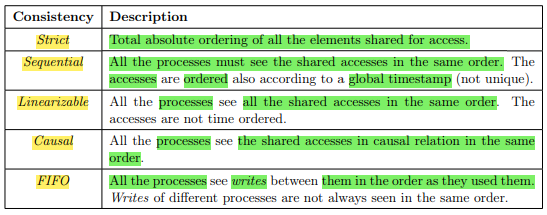
\includegraphics[width=.90\linewidth]{images/Replication/consistencyModelsTable1.png}
    \caption{Consistency models that don’t use synchronized operations}
\end{figure}

\begin{figure}[!h]
    \centering
    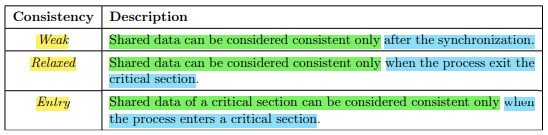
\includegraphics[width=.90\linewidth]{images/Replication/consistencyModelsTable2.png}
    \caption{Consistency models with synchronized operations}
\end{figure}

\subsection{Eventual Consistency}
Eventual consistency is \textbf{client centered}, it guarantees the correct access to the data store from the viewpoint of each client. It guarantee to propagate the update to all the copies at the end, it is efficient if the clients always work on the same replica.

There are different models that describe the access:
\begin{itemize}
    \item \textbf{Monotone reads:} if the process \textit{reads x}, every successive read of that process returns the same value or a more recent one
    \item \textbf{Monotone writes:} a \textit{write} of a process on \(x\) is completed before any other write on x of the same process
    \item \textbf{Read your write:} the effects of a \textit{write} on \(x\) by a process are always visible by successive \textit{read} on \(x\) by the same process.
    \item \textbf{Write follow reads:} guarantees that a \textit{write} on \(x\) by a process successive to a \textit{read} on \(x\) by the same process gives the same results read or a more recent one.
\end{itemize}

\section{Replica Positioning}
The data in our system consist of a collection of items that we shall call objects. An \textit{Object} could be a file but remember that each logical object is implemented by a collection of physical copies cal. The replicas are physical objects, each stored at a single computer, with data and behavior that are tied to some degree of consistency by the system’s operation.

Replicas can be stored in memory in different ways:
\begin{itemize}
    \item \textbf{Permanent:} they are static copies
    \item \textbf{Server-initiated:} they are created dynamically
    \item \textbf{Client-initiated:} they are based on the client cache
\end{itemize}

\subsection{System model}
The model involves replicas held by distinct \textbf{replica managers}, which are software components that contain the replicas on a given computer and perform operations upon them directly. We shall always require that a replica manager applies operations to its replicas recoverably, in such a way that these operation can be \textbf{recovered}.

\begin{figure}[!h]
    \centering
    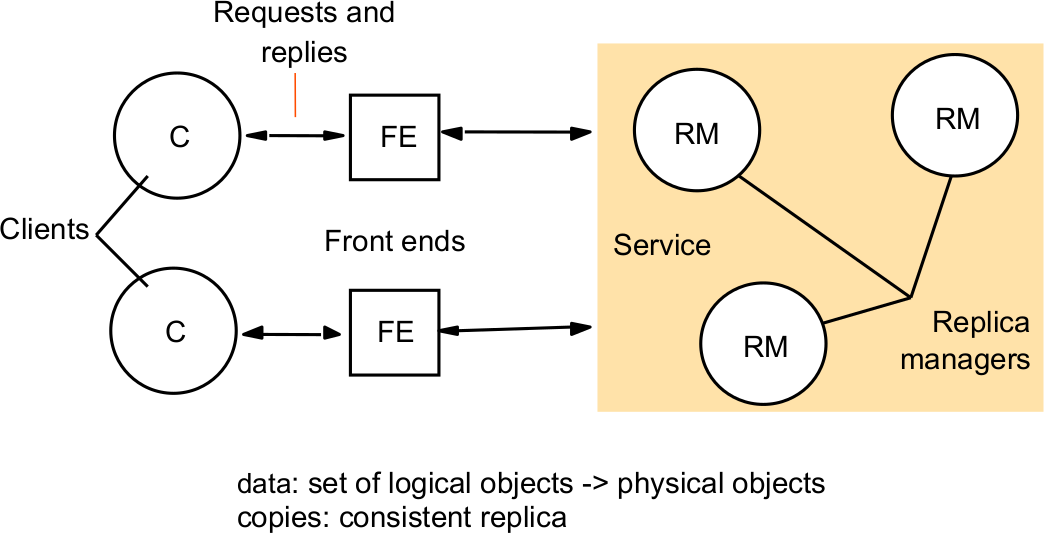
\includegraphics[width=.70\linewidth]{images/Replication/ArchitecturalModelReplicatedData.png}
    \caption{A basic architectural model for the management of replicated data}
\end{figure}

In the previous image it is possible to see the general model of replica management.
\begin{itemize}
    \item A collection of replica managers provides a service to clients
    \item The clients see a service that gives them access to objects, replicated by the managers
    \item Each client requests a series of operations
    \item Requested operations that involve \textbf{no updates} are called \textit{read-only requests}
    \item Requested operations that \textbf{update} an object are called \textit{update requests}
\end{itemize}

Each client’s requests are first handled by a component called a \textbf{front end}.
\begin{itemize}
    \item Its role is to communicate by message passing
    \item Front end introduces replication, location and access transparency
    \item A front end may be implemented in the client’s address space, or it may be a separate process.
\end{itemize}

In general, it is possible to highlight five steps during the execution of a single request upon replicated objects:
\begin{enumerate}
    \item \textbf{Request:} The front end issues the request to one or more replica managers in two possible ways:
    \begin{itemize}
        \item Either the front end communicates with a single replica manager, which in turn communicates with other replica managers.
        \item Or the front end multicast the request to the replica managers
    \end{itemize}
    \item \textbf{Coordination:} replica managers coordinate for executing the request consistently, they agree on whether the request is to be applied
    \begin{itemize}
        \item \textit{FIFO ordering:} if a front end issues request \(r\) and then request \(r'\)
        \item \textit{Casual ordering:} if the issue of request \(r\) happened-before the issue of request \(r'\)
        \item \textit{Total ordering:} if a correct replica manager handles \(r\) before request \(r'\)
    \end{itemize}
    \item \textbf{Execution:} The replica managers execute the request, perhaps \textit{tentatively}, in order to undo its effects later
    \item \textbf{Agreement:} The replica managers reach consensus on the effect of the request, if they agree to the commit choice, that will be committed
    \item \textbf{Response:} One or more replica managers responds to the front end.
\end{enumerate}